\documentclass[12pt,letterpaper]{article}
\usepackage[utf8]{inputenc}
\usepackage[spanish]{babel}
\usepackage{graphicx}
\usepackage[left=2cm,right=2cm,top=2cm,bottom=2cm]{geometry}
\usepackage{graphicx} % figuras
% \usepackage{subfigure} % subfiguras
\usepackage{float} % para usar [H]
\usepackage{amsmath}
%\usepackage{txfonts}
\usepackage{stackrel} 
\usepackage{multirow}
\usepackage{enumerate} % enumerados
\renewcommand{\labelitemi}{$-$}
\renewcommand{\labelitemii}{$\cdot$}
% \author{}
% \title{Caratula}
\begin{document}

% Fancy Header and Footer
% \usepackage{fancyhdr}
% \pagestyle{fancy}
% \cfoot{}
% \rfoot{\thepage}
%

% \usepackage[hidelinks]{hyperref} % CREA HYPERVINCULOS EN INDICE

% \author{}
\title{Caratula}

\begin{titlepage}
\begin{center}
\large{UNIVERSIDAD PRIVADA-DE-TACNA}\\
\vspace*{-0.025in}
\begin{figure}[htb]
\begin{center}

\includegraphics[width=8cm]{./Imagenes/logo}
\end{center}
\end{figure}
\vspace*{0.15in}
INGENIERIA DE SISTEMAS  \\

\vspace*{0.5in}
\begin{large}
TITULO:\\
\end{large}

\vspace*{0.1in}
\begin{Large}
\textbf{INFORME DE LABORATORIO No 05} \\
\end{Large}

\vspace*{0.3in}
\begin{Large}
\textbf{CURSO:} \\
\end{Large}

\vspace*{0.1in}
\begin{large}
BASE DE DATOS II\\
\end{large}

\vspace*{0.3in}
\begin{Large}
\textbf{DOCENTE(ING):} \\
\end{Large}

\vspace*{0.1in}
\begin{large}
 Patrick Cuadros Quiroga\\
\end{large}

\vspace*{0.2in}
\vspace*{0.1in}
\begin{large}
Integrantes: \\
\begin{flushleft}
Arlyn Cotrado Coaquira		\hfill	(2016054466) \\
Yaneth Virginia Aquino Huallpa		\hfill	(2017059286) \\
Sharon Sosa Bedoya            	\hfill	(2016054460) \\
Marlon Villegas Arando	\hfill	(2015053890) \\
\end{flushleft}
\end{large}
\end{center}

\end{titlepage}


\tableofcontents % INDICE
\thispagestyle{empty} % INDICE SIN NUMERO
\newpage
\setcounter{page}{1} % REINICIAR CONTADOR DE PAGINAS DESPUES DEL INDICE

\section{INFORMACIÓN GENERAL} 

\begin{itemize}
\subsection{Objetivos:}
	\item Conocer los fundamentos sobre como realizar una Gestion de Base de Datos con Oracle.
	\item Poder instalar correctamente una instancia.
\subsection{Equipos, materiales, programas y recursos utilizados:}
	\item Virtualización activada en el BIOS.
	\item Windows 10 64bit: Pro, Enterprise o Education, con al menos 4GB de RAM.
	\item Docker Desktop
	\item Oracle SQL Developer para Windows
	\item Microsoft SQL Server 2017 o superior

\end{itemize}

\section{MARCO TEORICO} 

\begin{itemize}
\subsection{ Docker:}
	\item Tener un docker que provea el gestor de base de datos es muy útil porque se reducen tiempos de instalación y configuración y en caso de tener un error muy grave en la configuración es tan sencillo resolverlo como borrar el contenedor y crear uno nuevo.
          \item Los contenedores funcionan bien para desarrollo y tal vez algunos ambientes de evaluación para el cliente, pero para ambientes productivos para nada se recomiendan, en estos casos siempre será lo mejor que se cuente con una base de datos instalada en el servidor.
         \item Sirven para desplegar aplicaciones en un entorno virtual aislado, pero sin el overhead de tener un Sistema Operativo (SO) nuevo como se tiene en una Virtual Machine (VM).

\subsection{Oracle Database en Docker:}
	\item Los productos de Oracle son compatibles con Docker si el sistema operativo del host es Oracle Linux 7, pero no necesita usar un host OL7 para que esto funcione. Puedes ver cómo instalar Docker en OL7 .
	\item Usar imágenes de Oracle Container Registry o de Docker Store tiene la ventaja que los binarios de instalación vienen incluidos, lo que no es permitido por licencia en el resto de las distribuciones. 
\subsection{Referencias de cómo usar Oracle con Docker en Linux Y  en Windows:}
	\item Docker en Windows 10:
	\item Para usar la versión completa es necesario habilitar Microsoft Hyper-V, lo que implica deshabilitar la virtualización por hardware de nuestro PC. Si estamos usando VirtualBox en el mismo host, con este cambio deja de funcionar.
Docker Toolbox no tiene esta restricción, aunque se mantiene como una versión antigua (Legacy), y Docker recomienda usar la versión completa.Otra diferencia de Docker Toolbox es que necesita una VM VirtualBox para ejecutar. Esta VM se crea de forma automática al usar Toolbox, de nombre default, y se usa como host para los containers que creemos.
 \subsection{Construir la imagen:}
	\item La compilación espera el siguiente sistema de archivos. Tendrá que descargar la base de datos Oracle 19c y el software APEX usted mismo y colocarlo en el directorio "software".
                     \begin{figure}[H]
		\begin{center}
		\includegraphics[width=8cm]{./Imagenes/100}
		\end{center}
		\end{figure}
	

\end{itemize}








\section{PROCEDIMIENTO} 

\begin{itemize}
\subsection{Parte 1: Conectar a SQL Server desde Power BI Desktop }
	\item Para realizar los gráficos en PowerBi Desktop primero debemos conectarnos con nuestra base de datos, que ya tiene que tener la base de datos "AdventureWorks 2017".  \\Abrimos nuestro PowerBi desktop y procedemos a realizar la conexión a SQL server.
	\begin{figure}[h]
	\begin{center}
	\fbox{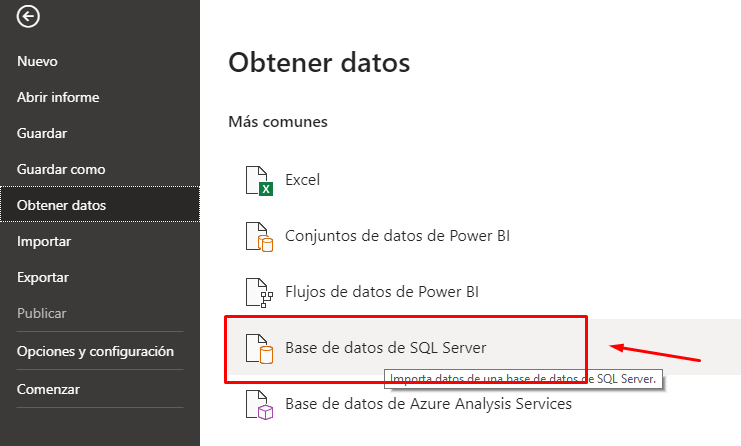
\includegraphics[width=12cm]{./Imagenes/tarea1}}
	\end{center}
	\end{figure}

\begin{figure}[h]
	\begin{center}
	\fbox{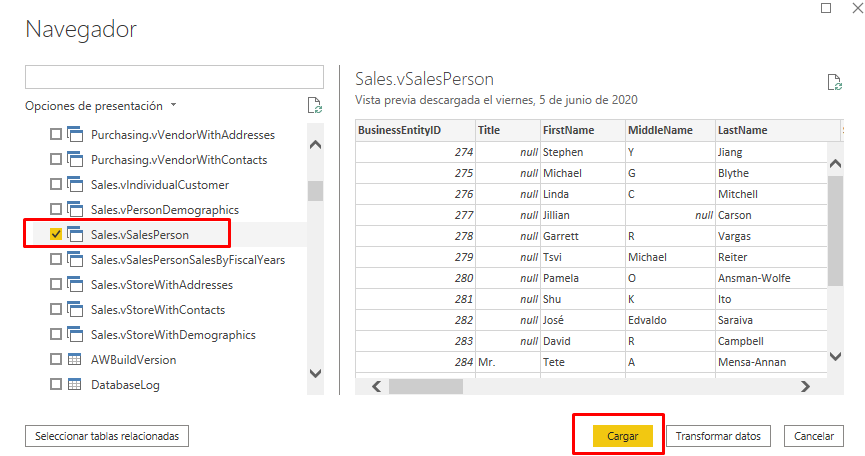
\includegraphics[width=13cm]{./Imagenes/tarea1_1}}
	\end{center}
	\end{figure}
\clearpage
	\begin{figure}[h]
	\begin{center}
	\fbox{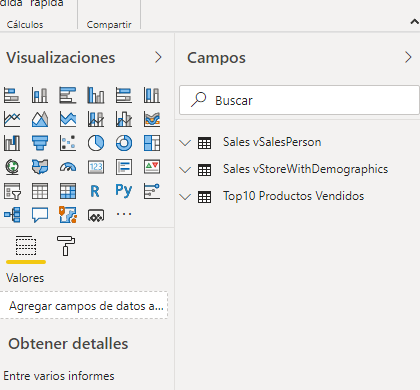
\includegraphics[width=11cm]{./Imagenes/tarea1_2}}
	\end{center}
	\end{figure}

	\item Una vez terminado de cargas los datos que necesitaremos, podremos visualizarlo en el panel lateral derecho de nombre "Campos".
	
     
\subsection{Parte 2: : Adicionar Gráficos al Reporte}
	\item En la parte 2 realizaremos los gráficos con la información de la base de datos que seleccionamos. Utilizaremos del panel de Visualizaciones los diferentes gráficos que nos ofrecen.

\begin{itemize}
	\item{\textbf{1. Cantidad de Ventas del personal: }} Gráfico de Columna Apilada que nos muestra el reporte de la cantidad de ventas de cada personal de ventas.
	\item {\textbf{2. Número de Empleados por especialidad: }}En el gráfico de Pie, muestra los la cantidad de empleados que tiene la empresa según su especialidad.
	\item {\textbf{3. Top 10 Productos vendidos: }}El gráfico de Donut, muestra el top 10 de los productos más vendidos. Podremos visualizarlo representados en los diferentes colores en el gráfico.
	\item {\textbf{4. Ventas Anuales y Beneficios Anuales: }}En el segundo gráfico de Columna Apilada podremos visualizar la cantidad de ventas anuales y los beneficios que ha traido. 
	\end{itemize}

\begin{figure}[h]
	\begin{center}
	\fbox{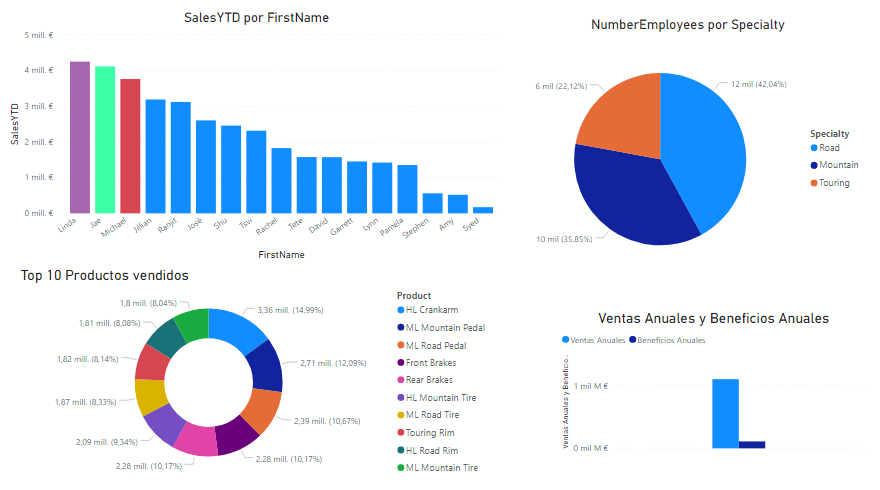
\includegraphics[width=15cm]{./Imagenes/tarea2}}
	\end{center}
	\end{figure}
		
\clearpage

\subsection{Parte 3: Publicar el reporte en el portal de Power BI}
	\item Cuando los gráficos esten listos, seleccionamos la opción de "Publicar" que nos ofrece PowerBi y poder subirlo a nuestra "Área de Trabajo". Cuando damos a "Aceptar" el archivo se irá subiendo a nuestra cuenta.

\begin{figure}[h]
	\begin{center}
	\fbox{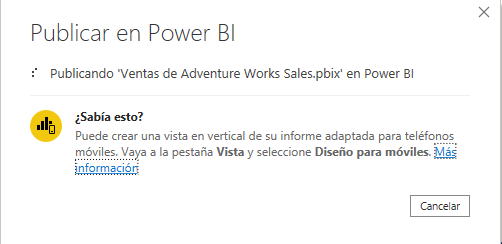
\includegraphics[width=11cm]{./Imagenes/tarea3}}
	\end{center}
	\end{figure}

\item Una vez se haya terminado de subir, abrimos nuestra cuenta desde la página web de Microsoft PowerBi y podremos visualizar nuestro trabajo ahí.

\begin{figure}[h]
	\begin{center}
	\fbox{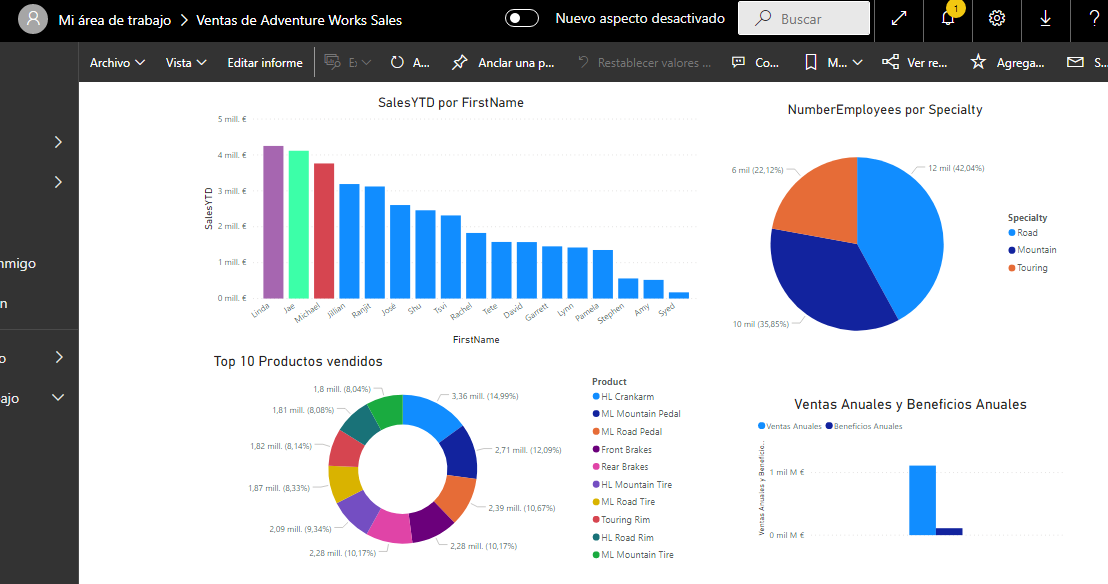
\includegraphics[width=14cm]{./Imagenes/tarea3_1}}
	\end{center}
	\end{figure}

\end{itemize}
		
\section{ANALISIS E INTERPRETACION DE RESULTADOS} 


\subsection{Parte 1: Actividades Encargadas}
	\begin{itemize}
		\item ¿Con qué comando(s) puedo iniciar y detener una instancia de Oracle, detalle cada uno de los pasos y opciones,
utilizando Docker?
                     \item Para  Iniciar una instancia de Oracle Database Server
Iniciar una instancia de servidor de base de datos Oracle al ejecutar
" docker run -d -it --name oracle-db store/oracle/database-enterprise:12.2.0.1"donde oracle01-db está el nombre del contenedor y 12.2.0.1 es la etiqueta de imagen de Docker.
                      \begin{figure}[H]
		\begin{center}
		\includegraphics[width=15cm]{./Imagenes/200}
		\end{center}
		\end{figure}
                      \item Los comandos docker ps -a -q detendrá todos los contenedores Docker en ejecución :
                      \begin{figure}[H]
		\begin{center}
		\includegraphics[width=15cm]{./Imagenes/201}
                      \includegraphics[width=8cm]{./Imagenes/202}
		\end{center}
		\end{figure}
		\item ¿Con qué comando(s) puedo iniciar y detener el Listener y el Enterprise manager, detalle cada uno de los pasos y
opciones, utilizando Docker?
                     \item Parar iniciar el listener:" lsnrctl start"  para detener "lsnrctl stop"
                      \begin{figure}[H]
		\begin{center}
		\includegraphics[width=15cm]{./Imagenes/203}
                      \includegraphics[width=15cm]{./Imagenes/204}
		\end{center}
		\end{figure}
		\item Genere un nuevo contenedor y cree un espacio de tablas con las siguientes características.
		\begin{figure}[H]
		\begin{center}
		\includegraphics[width=8cm]{./Imagenes/t3}
		\includegraphics[width=15cm]{./Imagenes/23}
		\end{center}
		\end{figure}


	\end{itemize}




\section{CONCLUSIONES}
Como podemos apreciar, hoy tenemos una tecnología disponible desde hace unos años que nos permite ir a otro nivel de virtualización distinto, permitiéndonos obtener las siguientes ventajas:
\begin{itemize}
\item Instalación simple y capacidad de ejecutar múltiples aplicaciones en entornos aislados sobre un mismo sistema operativo,  permitiéndonos ahorrar horas de trabajo en la administración de Infraestructura.
\item Independiente a la plataforma, permite contar con soluciones más portables.
\item Despliegue de Aplicaciones mucho más rápida y flexible.
\item Disponible en múltiples proveedores de Nube.
	
\end{itemize}

\newpage

\section{REFERENCIAS} 

\begin{itemize}
	\item [[ 1]] Hat, R. (2017). ¿Qué es Docker?. Recuperado de https://www.redhat.com/es/topics/containers/what-is-docker
	\item [[ 2]] código chido. (2019). Docker Oracle. Recuperado de https://https://codigochido.com/post/2019-01-21-docker-oracle/
         \item [[ 3]] Nelson, C. (2018). Usando Oracle 12c en Docker sobre Windows 10. Recuperado de https://https://www.oracle.com/technetwork/es/articles/datawarehouse/oracle12c-docker-win10-4485487-esa.html
         \item [[ 4]] The ORACLE-BASE Blog. (2018). Oracle Database en Docker. Recuperado de https://https://oracle-base.com/articles/linux/docker-oracle-database-on-docker
\end{itemize}




\end{document}
